\chapter{文献阅读理解}
\label{chap:2}

\section{基于 GAN 的图像生成模型}


%\begin{Verbatim}
%Attention Is All You Need
%\end{Verbatim}

\subsection{朴素 GAN 的基本模型}

生成对抗网络(Generative adversarial network, GAN)自2014年由Ian Goodfellow等人提出后,就越来越受到学术界和工业界的重视。而随着GAN在理论与模型上的高速发展,它在计算机视觉、自然语言处理、人机交互等领域有着越来越深入的应用,并不断向着其它领域继续延伸。其中,GAN在图像生成上取得了巨大的成功,这取决于GAN在博弈下不断提高建模能力,最终实现以假乱真的图像生成。

GAN受博弈论中的零和博弈启发,将生成问题视作判别器和生成器这两个网络的对抗和博弈:生成器从给定噪声中(一般是指均匀分布或者正态分布)产生合成数据,判别器分辨生成器的的输出和真实数据。前者试图产生更接近真实的数据,相应地,后者试图更完美地分辨真实数据与生成数据。由此,两个网络在对抗中进步,在进步后继续对抗,由生成网络得到的数据也就越来越完美,逼近真实数据,从而可以生成想要得到的数据(图片、序列、视频等)。

GAN包含有两个模型,一个是生成模型(generative model),一个是判别模型(discriminative model)。生成模型的任务是生成看起来自然真实的、和原始数据相似的实例。判别模型的任务是判断给定的实例看起来是自然真实的还是人为伪造的(真实实例来源于数据集,伪造实例来源于生成模型)。

\begin{figure}[htb]
\centering 
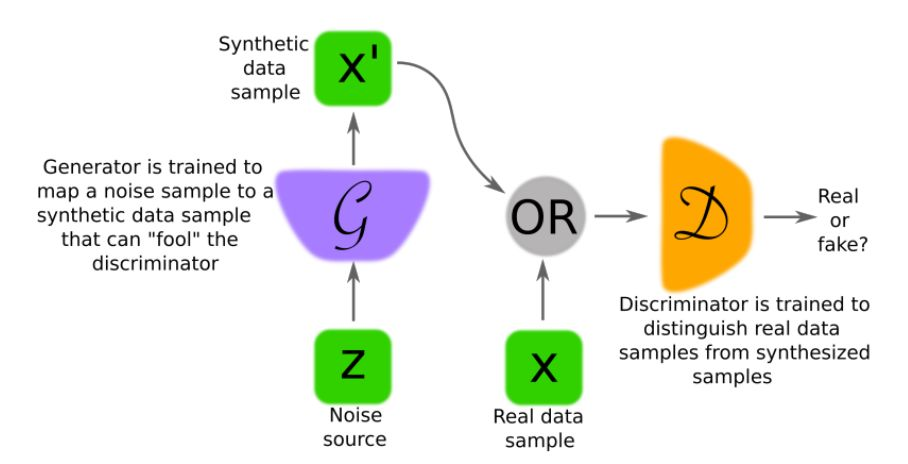
\includegraphics[width=0.8\textwidth]{img/m2t1.png} 
\caption{GAN 的基本结构}
\label{Test}
\end{figure}

理论上GAN可以将任意的分布作为输入,如上图所示,输入 z 为随机噪声,在实验中此研究多取 $z∼(0,1)$ 或 $z∼[-1,1]$ 的均匀分布作为输入。生成器 G 的参数为 $\theta$,输入 z 在生成器下得到 $x^\prime=G(z;\theta)$,输出可以被视为从分布中抽取的样本 $G(z; \theta)∼ p_{g}$ 。对于训练样本 x 的数据分布为 $p_{data}$ ,生成器 G 的目标是使 $p_{g}$ 近似$p_{data}$ ,判别器 D 的目标则是尽可能区分生成样本和真实样本的真假,通过最大-最小博弈来进行训练,这种博弈可公式化为:

\begin{equation}
\min \max V(D, G)=E_{x \square p_{\text {data }}(x)}[\log D(x \mid y)]+E_{z \square p_{z}(z)}[\log (1-D(G(z \mid y)))]
\end{equation}

%\begin{figure}[htb]
%\centering 
%\includegraphics[width=0.6\textwidth]{img/tm1.png} 
%\caption{The Transformer - 模型架構 (model architecture)}
%\label{Test}
%\end{figure}

其中第一项的 $logD(x)$ 表示判别器对真实数据的判断,第二项 $log(1\ -\ D(G(z)))$ 表示对合成数据的判断。通过这样一个最大最小 $(Max-min)$ 博弈,循环交替地分别优化G和D来训练所需要的生成式网络与判别式网络,直到到达 Nash 均衡点。

\subsection{GAN 的优缺点}

优势 :

\begin{enumerate}
 \item 根据实际的结果,GAN看上去可以比其它模型产生更好的样本(图像更锐利、清晰)。
 \item 生成对抗式网络框架能训练任何一种生成器网络(这是理论上的 ,而实践中,用 REINFORCE 来训练带有离散输出的生成网络非常困难)。大部分其他的框架需要该生成器网络有一些特定的函数形式,比如输出层是高斯的。
 \item 不需要设计遵循任何种类的因式分解的模型,任何生成器网络和任何鉴别器都会有用。
 \item 无需利用马尔科夫链反复采样,无需在学习过程中进行推断(Inference),回避了近似计算棘手的概率的难题。
\end{enumerate}

劣势 :

\begin{enumerate}
 \item 判别器越好,生成器的梯度消失越严重,这样会导致在网络训练上很多时候生成器的参数基本上不会发生改变。
 \item 由于网络是对抗式的,常常会造成训练时模型的崩溃(collapse mode),在训练时往往需要权衡训练的生成器与鉴别器的参数来防止崩溃的发生。这样在实际的应用上也带了很多不便。
\end{enumerate}

%\begin{enumerate}
% \item 
% \item 
% \item 
% \item 
%\end{enumerate}

\subsection{GAN 的一些经典变种}

1. DCGAN:

其论文名为 Unsupervised Representation Learning with Deep Convolutional Generative Adversarial Networks ,而 DCGAN 是继 GAN 之后比较好的改进,其主要的改进主要是在网络结构上,到目前为止,DCGAN的网络结构还是被广泛的使用,DCGAN极大的提升了GAN训练的稳定性以及生成结果质量。

DCGAN 对上述的 G 和 D 用了两个卷积神经网络(CNN),同时对卷积神经网络的结构做了一些改变,以提高样本的质量和收敛的速度,这些改变有取消所有 pooling 层。G网络中使用转置卷积(transposed convolutional layer)进行上采样,D网络中用加入stride的卷积代替 pooling;在 D 和 G 中均使用 batch normalization;去掉 FC 层,使网络变为全卷积网络;G 网络中使用 ReLU 作为激活函数,最后一层使用 tanh;D 网络中使用 LeakyReLU 作为激活函数。

\begin{figure}[htb]
\centering 
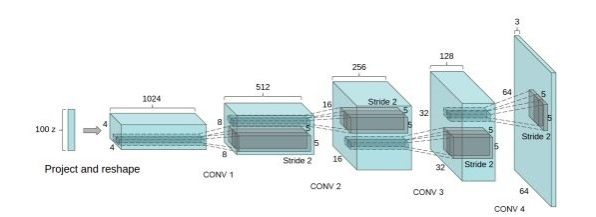
\includegraphics[width=0.8\textwidth]{img/m2t2.jpg} 
\caption{DCGAN}
\label{Test}
\end{figure}

2. WGAN 和 WGAN-GP

WGAN 也是一篇经典,其名為 Wasserstein GAN,WGAN 主要从损失函数的角度对 GAN 做了改进,损失函数改进之后的 WGAN 即使在全链接层上也能得到很好的表现结果,具体的来说,WGAN 对GAN的改进有判别器最后一层去掉 sigmoid;生成器和判别器的loss不取log;对更新后的权重强制截断到一定范围内,比如[-0.01,0.01],以满足论文中提到的lipschitz连续性条件;论文中也推荐使用SGD,RMSprop等优化器,不要基于使用动量的优化算法,比如 adam。

而 WGAN-GP 论文为 Improved Training of Wasserstein GANs 之前的 WGAN 虽然理论上有极大贡献,但在实验中却发现依然存在着训练困难、收敛速度慢的问题,这时 WGAN-GP 被提出来,它的贡献是提出了一种新的 lipschitz 连续性限制手法—梯度惩罚,解决了训练梯度消失梯度爆炸的问题;比标准 WGAN 拥有更快的收敛速度,并能生成更高质量的样本;提供稳定的 GAN 训练方式,几乎不需要太多调参,成功训练多种针对图片生成和语言模型的 GAN 架构。

\subsection{GAN 图像生成}

根据不同的GAN所拥有的生成器和判别器的数量,可以将 GAN 图像生成的方法概括为三类:直接方法,迭代方法和分层方法。

\begin{figure}[htb]
\centering 
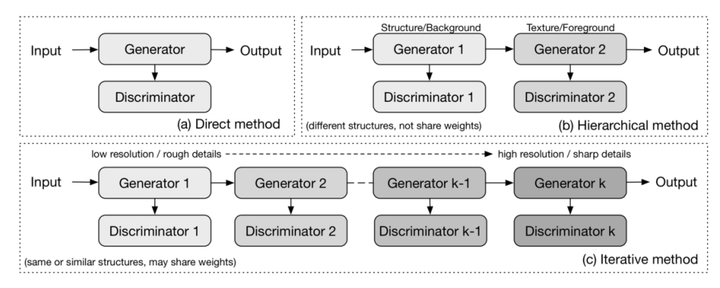
\includegraphics[width=0.8\textwidth]{img/m2t3.png} 
\caption{GAN 图像生成}
\label{Test}
\end{figure}

1. 直接法

早期的GANs都遵循在其模型中使用一个生成器和一个判别器的原理,并且生成器和判别器的结构是直接的,没有分支。如GAN、DCGAN、ImprovedGAN,InfoGAN,f-GAN和GANINT-CLS。这类方法在设计和实现上比较容易,通常也能得到良好的效果。

2. 分层法

分层法的主要思想是将图像分成两部分,如“样式和结构”和“前景和背景”,然后在其模型中使用两个生成器和两个鉴别器,其中不同的生成器生成图像的不同部分,然后再结合起来。两个生成器之间的关系可以是并联的或串联的。
以SS-GAN为例,其使用两个GAN,一个Structure-GAN用于生成表面结构,然后再由Style-GAN补充图片细节,最后生成图片,整体结构如下所示:

\begin{figure}[htb]
\centering 
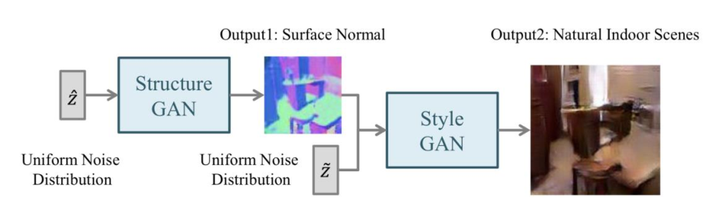
\includegraphics[width=0.8\textwidth]{img/m2t4.png} 
\caption{SS-GAN 的分层结构}
\label{Test}
\end{figure}

3. 迭代法

迭代法使用具有相似或甚至相同结构的多个生成器,经过迭代生成从粗到细的图像,而以 LAPGAN 为例,LAPGAN 中的多个生成器执行相同的任务:最低级别的生成器仅将噪声向量作为输入并输出图像,而其他生成器都从前一个生成器获取图像并将噪声矢量作为输入,这些生成器结构的唯一区别在于输入/输出尺寸的大小,每一次迭代后的图像都拥有更多清晰的细节。

\begin{figure}[htb]
\centering 
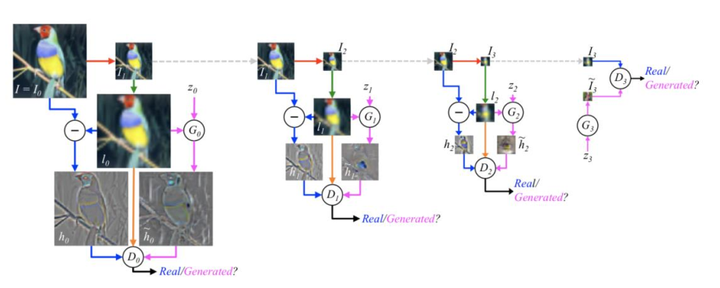
\includegraphics[width=0.8\textwidth]{img/m2t5.png} 
\caption{LAPGAN 的迭代结构}
\label{Test}
\end{figure}

\section{条件图像生成}

如果 GAN 的生成器和判别器可以以某些额外的信息为条件,而非仅仅由正态采样的噪声控制生成,那么生成对抗网就可以扩展到条件模型。类似于条件概率,设y是任何类型的条件信息,如文本或其他形式的图像,该研究可以通过将y作为噪声z之外的附加信息输入判别器和生成器,引导生成效果。而将条件信息加入生成器和判别器中又分为两种情况:(1).原始生成对抗网络的生成器的输入是噪声信号,从而类别标签可以和噪声信号组合作为隐藏空间表示;(2).原始生成对抗网络的判别器输入是图像数据(真实图像和生成图像),同样需要将类别标签和图像数据进行拼接作为判别器输入。
从而生成对抗网络的目标函数变为:

\begin{equation}
\min \max V(D, G)=E_{x \square p_{\text {data }}(x)}[\log D(x \mid y)]+E_{z \square p_{z}(z)}[\log (1-D(G(z \mid y)))]
\end{equation}

条件生成对抗网络的网络结构相对于原始生成对抗网络并没有变化,改变的仅仅是生成器和判别器的输入数据,这就使得 CGAN 可以作为一种通用策略嵌入到其它的GAN网络中。经典的条件图像生成 GAN 网络有两种:

\subsection{Image-to-Image Translation with Conditional Adversarial Networks}

图像处理、计算机图形学和计算机视觉中的许多问题都可以归结为将输入图像“翻译”成相应的输出图像的问题。正如任何一种概念都可以用英语或法语表达一样,场景也可以被渲染为RGB图像、梯度场、边缘图、语义标签图等。与自动语言翻译问题类似,此研究将图像到图像的翻译问题定义为在给定足够的训练数据的情况下,将一个场景的一种可能表示翻译成另一种可能表示的问题。传统上,尽管这些任务都可以概括为从像素到像素的预测,但这些任务中的每一种都是用特定的方法处理的。而pix2pix的提出为解决这些问题提出了一个通用的框架。

1. 模型结构

pix2pix 的生成器采用 U-Net 结构,将输入原始图像编码再解码成另一种风格图像,从而实现图像翻译。判别器使用 PatchGAN 结构,作用为在输入原始图像的条件下,对于生成的图片判断为假,对于真实图片判断为真。生成器使用U-Net结构的原因主要在于对于图像翻译问题,输入和输出图像的纹理应该不同,但潜在的内容结构应该相似,这就需要生成器的输入和输出共享一些底层的信息,因此生成器使用 U-Net ,因为它采用了跳越连接(skip-connection)的方法对编码器和解码器共享底层信息。

\begin{figure}[htb]
\centering 
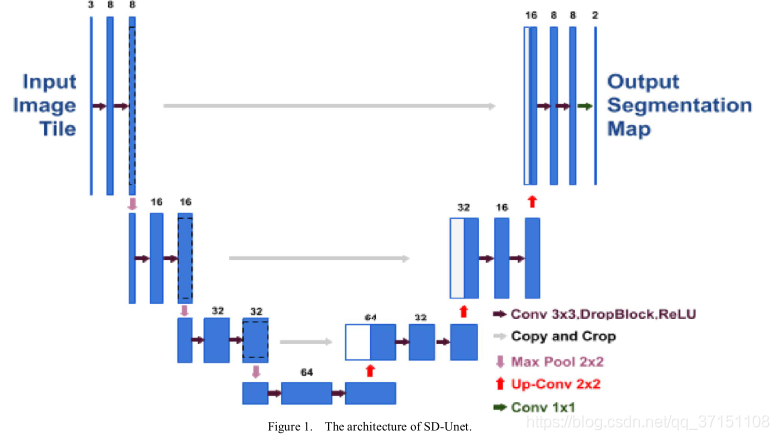
\includegraphics[width=0.8\textwidth]{img/m2t6.png} 
\caption{模型结构}
\label{Test}
\end{figure}

判别器使用 PatchGAN 的结构的原因在于采用 L1 损失和 L2 损失进行重建会导致图像模糊,也就是说 L1 损失和 L2 损失并不能很好的恢复图像的高频部分,但能较好地恢复图像的低频部分。为了能更好得对图像的局部做判断, pix2pix 的判别器采用 patchGAN 的结构,也就是在判别过程中把图像等分成小块(patch),分别判断每个小块的真假,最后再取平均,得到的均值就是判别器对图像真伪的评分。文中提出的 PatchGAN 可以看成另一种形式的纹理损失。

\begin{figure}[htb]
\centering 
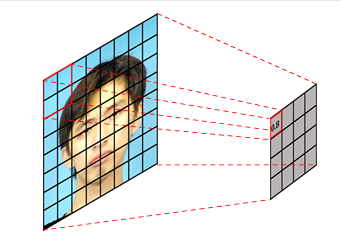
\includegraphics[width=0.8\textwidth]{img/m2t7.png} 
\caption{原始 GAN 的判别器}
\label{Test}
\end{figure}

原始 GAN 的判别器仅对整张输入图像输出一个评分,而 PatchGAN 使用卷积将输入映射为 $nXn$ 的评分矩阵,矩阵中每个元素对应原始图像中的一块小区域的评分,对评分矩阵求平均即得到整张图像的评分。这种计算方法能够更好地考察图像的细节,极大提升了判别器的性能。

2. 损失函数

生成对抗网络其实就是一种相对于 L1 损失更好的判别准则或者说损失函数。一些情况下单独使用对抗损失效果更好,一些情况下对抗损失与 L1 损失配合起来效果更好。在 pix2pix 中,作者将L1损失和对抗损失结合使用,因为作者认为L1损失可以恢复图像的低频部分,而对抗损失可以恢复图像的高频部分,二者结合起来能够达到更好的生成效果。Pix2Pix 的损失函数公式为:

\begin{equation}
\min V_{G A N}+\alpha V_{L 1}
\end{equation}

\subsection{Unpaired Image-to-Image Translation using Cycle-Consistent Adversarial Networks}

图像到图像翻译的目标是使用样本为对齐图像对的训练集来学习输入图像和输出图像之间的映射。然而,对于许多任务,成对的训练数据是不易获取的。为了解决这一问题,pix2pix 的作者又提出了一种在没有成对样本的情况下学习将图像从源域X翻译到目标域Y的方法,这就是 CycleGAN。它的的目标是学习一个从X域到Y域的映射 ,使得来自的图像分布与使用对抗损失的分布\ Y 无法区分。因为这个映射是高度欠约束的,作者把它和一个逆映射 耦合起来,引入一个循环一致性损失 (Cycle consistancy loss) 来约束 $F\left(G\left(X\right)\right)=X$ (反之亦然)。这样就能在不存在成对训练数据的情况下, 完成不同风格域图像的翻译。

在模型结构上,CycleGAN 和 pix2pix 采用了相同的判别器(PatchGAN),但二者的生成器却略有不同。CycleGAN 的生成器采用类似于ResNet的跳跃连接结构,对图像下采样后用一系列残差块进行特征保持,再进行上采样。 CycleGAN 的主要创新为提出了循环一致性损失(Cycle Consistancy Loss),即同时训练两对生成器和判别器,最后用循环一致性损失对两对生成器和判别器进行约束,使它们学习到的映射为互相之间的逆映射。

\begin{figure}[htb]
\centering 
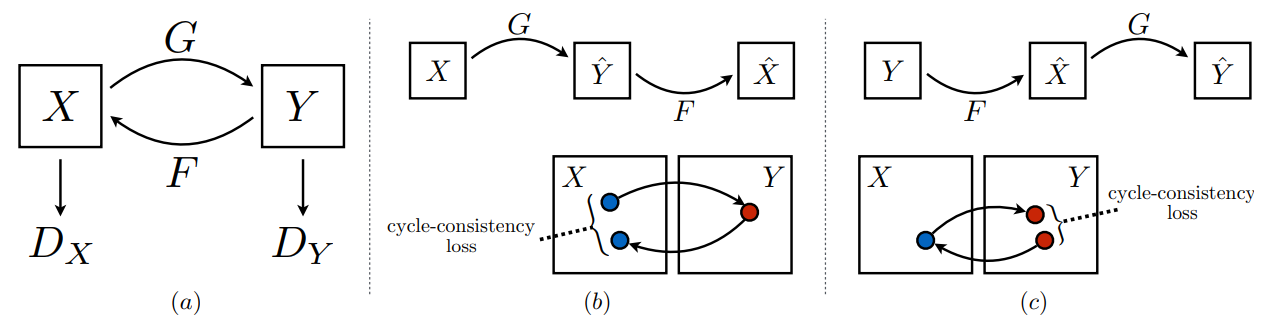
\includegraphics[width=0.8\textwidth]{img/m2t8.png} 
\caption{CycleGAN}
\label{Test}
\end{figure}

循环一致性损失用公式表述为:

\begin{equation}
V_{c y c}(G, F)=E_{x \square p_{\text {data }}(x)}\left[\|F(G(x))-x\|_{1}\right]+E_{y \square p_{\text {data }}(y)}\left[\|G(F(y))-y\|_{1}\right]
\end{equation}

\section{高分辨率图像生成}

\subsection{A Style-Based Generator Architecture for Generative Adversarial Networks}

1. Background

NVIDIA 在 2017 年提出的 ProGAN 解决了生成高分辨率图像(如1024×1024)的问题。ProGAN 的关键创新之处在于渐进式训练——从训练分辨率非常低的图像(如4×4)的生成器和判别器开始,每次都增加一个更高的分辨率层。

2. Motivation

与多数 GAN 一样,ProGAN 控制生成图像的特定特征的能力非常有限。这些属性相互纠缠,即使略微调整输入,会同时影响生成图像的多个属性。所以如何将 ProGAN 改为条件生成模型,或者增强其微调单个属性的能力,是一个可以研究的方向。

3. Contribution

(1) 借鉴风格迁移,提出基于样式的生成器(style-based generator)。

\begin{enumerate}
 \item [-] 实现了无监督地分离高级属性(人脸姿势、身份)和随机变化(例如雀斑,头发)
 \item [-] 实现对生成图像中特定尺度的属性的控制。
 \item [-] 生成器从一个可学习的常量输入开始,隐码在每个卷积层调整图像的“样式”,从而直接控制不同尺度下图像特征的强度。
\end{enumerate}

(2) 实现了对隐空间(latent space)较好的解耦。

生成器将输入的隐码z嵌入一个中间的隐空间。因为输入的隐空间Z必须服从训练数据的概率密度,这在一定程度上导致了不可避免的纠缠,而嵌入的中间的隐空间 W 不受这个限制,因此可以被解耦。

(3) 提出了两个新的量化隐空间解耦程度的方法

感知路径长度和线性可分性。与传统的生成器体系结构相比,新的生成器允许更线性、更解耦地表示不同的变化因素。

(4) 提出了新的高质量的人脸数据集(FFHQ,7万张1024×1024的人脸图片)

4. Framework

下图为 stylegan 生成器与传统GAN网络的对比。其中不同之处包括:

\begin{enumerate}
 \item [-] 移除了传统的输入(remove traditional input)
 \item [-] 映射网络(Mapping Network)
 \item [-] 样式模块(style modules,AdaIN,自适应实例归一化)
 \item [-] 随机变化(Stohastic variation,通过加入噪声为生成器生成随机细节)
\end{enumerate}

\begin{figure}[htb]
\centering 
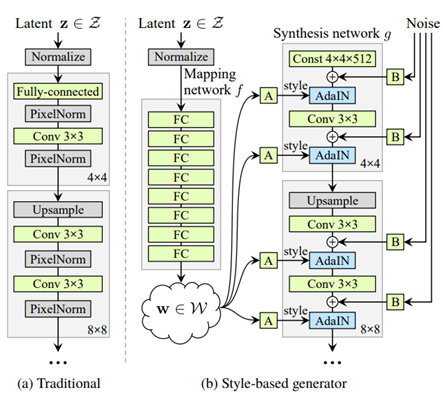
\includegraphics[width=0.8\textwidth]{img/m2t9.png} 
\caption{stylegan}
\label{Test}
\end{figure}

5. Results

(1) 生成的图像的质量

训练数据集分别是 CelelbA-HQ 和 FFHQ 。其中 FFHQ 数据集(本文提出的)Flickr-Faces-HQ(FFHQ),包含 7 万张高分辨率的人脸图像(2014×1024)。
评估指标为 FID(Fréchet Inception Distance,越小越好)。

\begin{figure}[htb]
\centering 
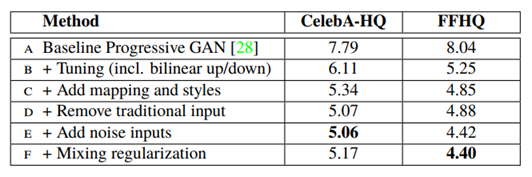
\includegraphics[width=0.8\textwidth]{img/m2t10.png} 
\caption{生成的图像的质量}
\label{Test}
\end{figure}

(2) 随机变化

显示了在相同底层图像输入不同的噪声实现的随机变化。噪声只影响随机方面,而保留了整体结构和身份、面部等高级特征。

\begin{figure}[htb]
\centering 
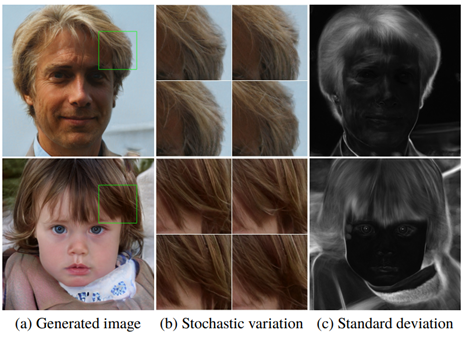
\includegraphics[width=0.8\textwidth]{img/m2t11.png} 
\caption{随机变化}
\label{Test}
\end{figure}

(3) 风格混合

\begin{figure}[htb]
\centering 
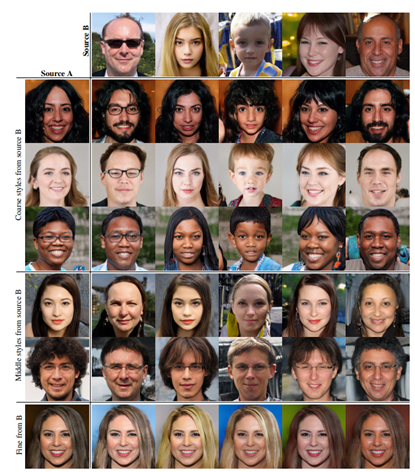
\includegraphics[width=0.8\textwidth]{img/m2t12.png} 
\caption{风格混合}
\label{Test}
\end{figure}

为了进一步鼓励样式进行本地化,采用混合正则化,即在训练过程中使用两个随机潜码而不是一个来生成给定百分比的图像。在生成这样的图像时,只需在合成网络中随机选择的位置从一个潜在代码切换到另一个潜在代码(称为样式混合的操作)。具体来说,通过映射网络运行两个潜在代码 z1,z2,并让相应的 w1,w2 控制样式,以便w1在交叉点之前应用,w2 在交叉点之后应用。这种正则化技术可防止网络假设相邻样式相关。

6. Conclusion

基于样式的生成器,能生成更高质量的高分辨率图像;实现了无监督地分离高级属性(人脸姿势、身份)和随机变化(例如雀斑,头发),实现对生成图像中特定尺度的属性的控制。通过 style 控制高级属性,通过不同层的 style 实现对不同尺度的特征的控制;通过噪声控制随机变化降低了隐空间的耦合性;通过映射网络生成中间隐空间(intermediate latent space),中间隐空间降低了输入隐空间的纠缠;提出两种新的量化隐空间耦合性的指标-感知路径长度和线性可分性;对高级属性与随机效应的分离以及中间隐空间的线性的研究,提高了对 GAN 合成的理解和可控性。

\subsection{Analyzing and Improving the Image Quality of StyleGAN}

该论文是 StyleGAN2 即在 StyleGAN 的基础上改进得到的。本文指出和分析了几个特征伪影,并在模型架构和训练方法上进行了调整以解决该问题。重新设计了生成器归一化,并正则化生成器以促进隐码到图像的映射有更好的条件。除了改善了图像质量,这个路径长度正则化器还带来了额外的好处,使得生成器更容易反转。本文进一步可视化生成器如何很好地利用其输出分辨率,并确定一个容量问题,激励该研究训练更大的模型,以获得额外的质量改进。该工作成为当时人脸生成领域的 SOTA,而本文主要贡献如下 :

1. 修复了 StyleGAN 中存在的水滴伪影

StyleGAN 生成的大多数图像都呈现出典型的水滴形状的人工伪影,即使液滴在最终图像中可能不明显,它也存在于生成器的中间特征图中。异常开始出现在64×64分辨率附近,出现在所有特征图中,并在更高分辨率时变得越来越强。
作者将问题定位于adaptive instance normalization (AdaIN) 操作,该操作分别对每个特征图的均值和方差进行归一化,有可能破坏了特征彼此之间的信息。而解决方法:A.改变网络结构  B. Weight demodulation。

2. 对渐进式增长进行修正

渐进生成器导致了相位问题。逐渐增长的生成器似乎对细节有强烈的偏好。当牙齿或眼睛等特征在图像上平滑移动时,它们可能会停留在原位。作者重新考虑了渐进式增长,提出了一种替代设计——训练从专注低分辨率的图像开始,然后逐步将焦点转移到高分辨率——在训练期间不改变网络拓扑。

3. PPL成为正则化项

Fréchet inception distance (FID) 和 Precision and Recall (P\&R)是生成图像质量量化评估的两大指标,这两个指标都是基于分类器网络的,专注于纹理而不是形状,不能准确地捕捉图像质量的所有方面。(perceptual path length; PPL)作为一种评估潜空间插值质量的一种方法,于形状的一致性和稳定性有关。在此基础上,本文对合成网络进行正则化,使其有利于平滑映射,并在质量上取得明显改进。为了抵消计算开销,作者还建议减少所有正则化的执行频率,不会影响其有效性。

4. 更大的容量

更大的模型进一步提高生成质量

(1) 新的网络架构

\begin{figure}[htb]
\centering 
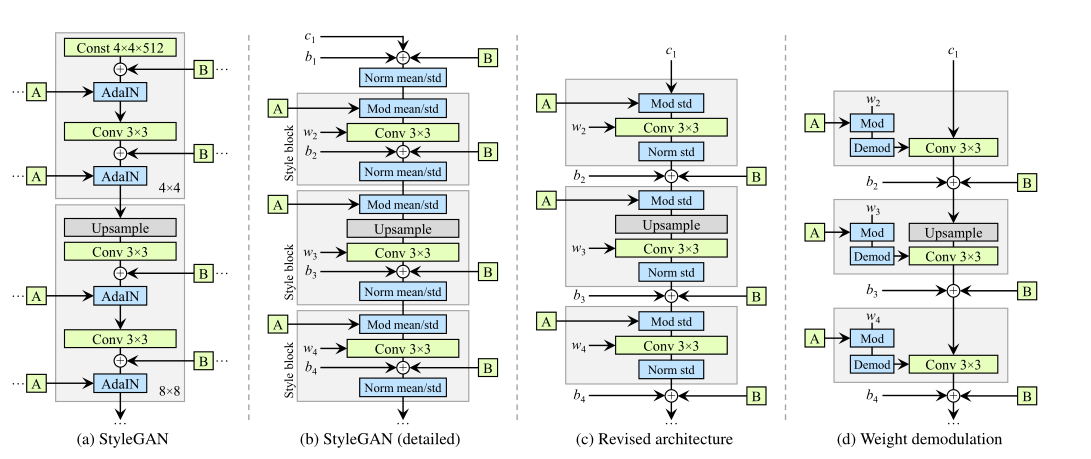
\includegraphics[width=0.9\textwidth]{img/m2t13.png} 
\caption{新的网络架构}
\label{Test}
\end{figure}

\begin{enumerate}
\item [-] 是原始的StyleGAN,其中 A 表示从 W 的一个仿射变换B是一个噪声广播操作。
\item [-] 更详细的 SyleGAN。通过显示权重和偏差,并将 AdaIN 操作分解为两个组成部分:归一化(normalization)和调制(modulation)。
\item [-] 对原始架构进行了调整修改。将b和B的相加移到了风格活动区域之外,可以获得更可预测的结果,并且只对标准差进行归一化(去掉了对均值的操作)。
\item [-] 修改后的架构使此研究能够用“解调”(demodulation)操作取代实例归一化,对特征图的修改改为对卷积权重的修改。
\end{enumerate}

(2) Weight demodulation

简单地去除归一化操作可以消除伪影,但是无法对风格混合(style mixing)有scale-specific级别的控制。本文提出了一个更好的方案能够在保留完全可控性的同时去掉伪影。将对特征图的一系列操作改为对权重的操作。特征图只经过卷积处理并添加噪声。缩放特征图改为缩放卷积权重(mod):

\begin{equation}
w_{i j k}^{\prime}=s_{i} \cdot w_{i j k}
\end{equation}

$s_{i}$ 是第i个输入特征图的缩放比例,经过缩放和卷积后,输出激活的标准差为:

\begin{equation}
\sigma_{j}=\sqrt{\sum_{i, k} w_{i j k}^{\prime}{ }^{2}}
\end{equation}

demod 权重,旨在使输出恢复到单位标准差:

\begin{equation}
w_{i j k}^{\prime \prime}=w_{i j k}^{\prime} / \sqrt{\sum_{i, k} w_{i j k}^{\prime}{ }^{2}+\epsilon}
\end{equation}

加一个 $\epsilon$ 避免分母为 0。

尽管这种方式与 Instance Norm 在数学上并非完全等价,但是 weight demodulation 同其它normalization 方法一样,使得输出特征图有着 standard 的 unit 和 deviation。

(3) 图像质量与生成器的平滑程度

作者观察发现更小的 perceptual path length (PPL) 有更高的整体图像质量。作者假设在训练过程中,由于鉴别器对破碎图像进行惩罚,对生成器进行改进最直接的方法是有效地拉伸产生良好图像的潜空间区域。这将导致低质量的图像被压缩到快速变化的小潜空间区域。虽然这可以在短期内提高平均输出质量,但累积的失真会损害训练状态,进而损害最终图像质量。

\begin{enumerate}
 \item [-] Lazy regularization : 每16个batch执行一次R1和路径长度正则化,大大降低计算成本和内存用量,而对结果无影响。
 \item [-] 路径长度正则化 : 无论 W 或图像空间方向如何,这些渐变应具有接近等长度,即小位移产生相同大小的变化。表示从潜在空间到图像空间的映射是良好的。路径长度正则化不但提高了图片的生成质量,而且使得生成器更平滑,生成的图片反转回 latent code 更容易了。
\end{enumerate}

\begin{figure}[htb]
\centering 
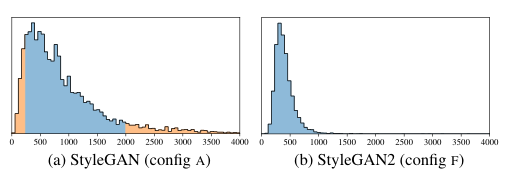
\includegraphics[width=0.9\textwidth]{img/m2t14.png} 
\caption{图像质量与生成器的平滑程度}
\label{Test}
\end{figure}

StyleGAN2(config F)极大地改善了 PPL 的分布,使之更加紧凑。但是结构化程度低于人脸 FFHQ 的 LSUN Car 数据集中的 FID 和 PPL 之间存在平衡。PPL 降低反而导致 FID 升高。如下图 config D 所示。

\begin{figure}[htb]
\centering 
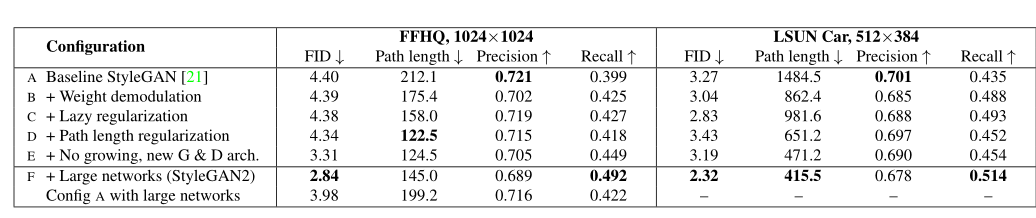
\includegraphics[width=0.9\textwidth]{img/m2t15.png} 
\caption{StyleGAN2}
\label{Test}
\end{figure}

(4) 渐进式增长修正

渐进增长在稳定高分辨率图像合成方面非常成功,但会产生特定的伪影,对细节有强烈的位置偏好。作者认为,在渐进增长的过程中,每个分辨率都会瞬间用作输出分辨率,迫使其生成最大频率细节,然后导致受过训练的网络在中间层具有过高的频率,从而损害了位移不变性。所以需要重新设计一个能产生高质量图像而不渐进增长的架构。 在生成方法的背景下,Skip connections,残差网络和分层方法也被证明是非常成功的。三种生成器(虚线上方)和判别器体系结构如下图。Up和Down分别表示双线性上和下采样。 在残差网络中,这些还包括1×1卷积以调整特征图的channel数。tRGB和fRGB在RGB和高维每像素数据之间转换。 Config E 和 F 中使用的体系结构以绿色突出显示。

\begin{figure}[htb]
\centering 
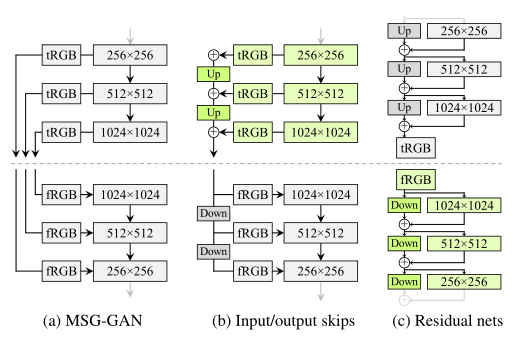
\includegraphics[width=0.9\textwidth]{img/m2t16.png} 
\caption{渐进式增长修正}
\label{Test}
\end{figure}

表下比较了三种生成器和三种鉴别器体系结果,StyleGAN 中使用的原始前馈网络、跳过连接和残差网络,它们都是未经渐进增长而训练的。

\begin{figure}[htb]
\centering 
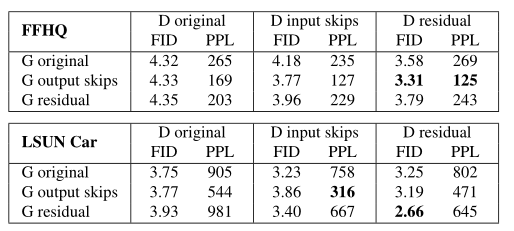
\includegraphics[width=0.9\textwidth]{img/m2t17.png} 
\caption{渐进式增长修正}
\label{Test}
\end{figure}

由上表可以看出使用 skips 连接的生成器 PPL 最小。使用残差网络的判别器对FID有利。StyleGAN2 使用了一个 skip generator 和一个残差鉴别器,切换到这种设置显著地改进了 FID 和 PPL 。

\begin{figure}[htb]
\centering 
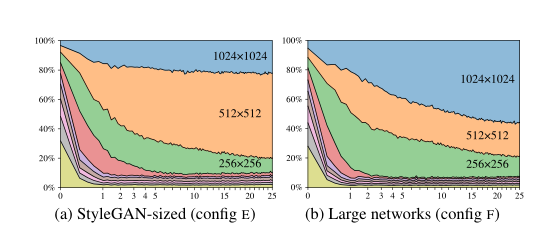
\includegraphics[width=0.9\textwidth]{img/m2t18.png} 
\caption{StyleGAN2}
\label{Test}
\end{figure}

从研究中可以看到,从一开始,网络就专注于低分辨率图像,并随着训练的进行逐渐将其注意力转移到较大分辨率上。在(a)中,生成器基本上输出 512x512 图像,并对 1024x1024 进行一些细微锐化。而在(b)中,较大的网络更多地关注高分辨率细节。通过将两个网络的最高分辨率层中的特征图的数量加倍来进行测试。这使行为更加符合预期:图(b)显示了贡献的显著增加,而实验结果如下。

\begin{figure}[htb]
\centering 
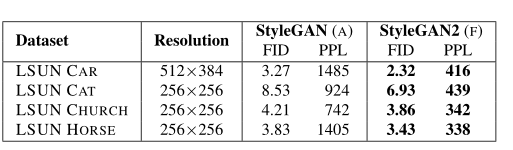
\includegraphics[width=0.9\textwidth]{img/m2t19.png} 
\caption{StyleGAN2}
\label{Test}
\end{figure}

该表在四个 LSUN 类别中对 StyleGAN 和 StyleGAN2 进行了比较,再次显示出FID的明显改善和 PPL 的显著进步。进一步扩大规模可能会带来额外的好处。

(5) 结论

本文确定和修复了StyleGAN中的几个图像质量问题,进一步提高了生成图像的质量。该论文的主要创新点如下:

\begin{enumerate}
 \item [-] 使用 Weight demodulation 代替 AdaIN。
 \item [-] 发现 PPL 与生成图像质量的关系,使用 Path length regularization。
 \item [-] 去除渐进式网络,在生成器和判别器中采用不同的网络结构。
\end{enumerate}

(6) 展望

在未来,研究路径长度正则化的进一步改进可能会带来成果,例如,用数据驱动的特征空间度量替换像素空间 $L_2$ 距离。而考虑到 GAN 的实际部署,寻找新的方法来减少训练数据需求是很重要的。在无法获取数万个训练样本的应用程序中,以及包含大量内在变化的数据集中,这一点尤其重要。

\subsection{Alias-Free Generative Adversarial Networks}

1. 研究背景

英伟达 StyleGAN 团队在 NeurIPS 2021 论文《 Alias-Free Generative Adversarial Networks 》中推出了 Alias-Free GAN,也即 StyleGAN3 。典型的 GAN 具有分层卷积性质,通过上采样层分层细化,随后经过卷积层进行局部混合,并经由非线性映射层引入新的细节,但它们的合成过程过度依赖于绝对像素坐标。这就导致图像细节会粘连在坐标上,而不在对象的表面,造成一种纹理粘连(texture sticking)的现象,例如下图,由 StyleGAN2 生成的毛发,主要都固定在相同的坐标上,导致了形成水平的条纹。

\begin{figure}[htb]
\centering 
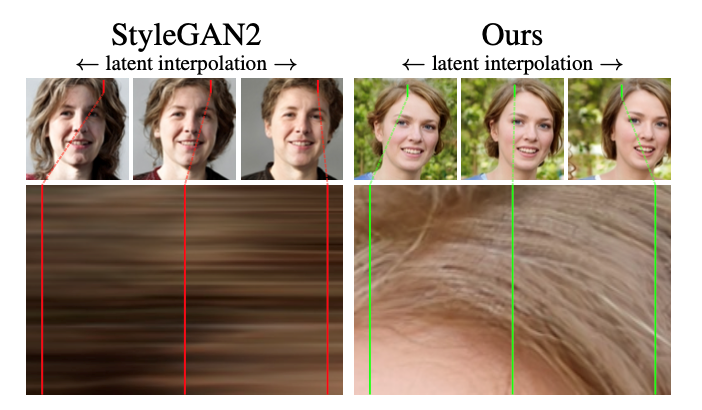
\includegraphics[width=0.9\textwidth]{img/m2t20.png} 
\caption{Alias-Free GAN}
\label{Test}
\end{figure}

因此英伟达的研究者探究导致 GANs 中文理粘连的现象,原因主要是“粗糙”的信号处理过程和神经网络混叠。而通过将网络中所有信号解读为连续性,他们进行了普遍适用的、小的架构变化,保证多余的信息不会参与分层合成过程,并由此得到了 StyleGAN3 与 StyleGAN2 相比,StyleGAN3 获得了类似的 FID,并在亚像素尺度上实现了真正的图像平移和旋转不变性,从而大幅度提升生成图像的质量。

2. 贡献

典型GAN生成器的结构化处理过程是:粗糙、低分辨率的特征通过上采样层分层细化,再通过卷积局部混合,以及非线性引入新的细节。这种体系结构可能基本还原了图像的表面特征,但它并没有以一种“自然而然”的方式合成更逼真的图像,也就是说,粗糙特征确保了图像细节的存在,但没有控制它们的精确位置,细节被固定在了图像坐标上。这项研究的目标就是,创建更自然的转换层次的体系结构,让每个特征的精确亚像素位置都从底层粗特征中获得。

本次则主要针对平移和旋转的两种类型移动,Alias-Free-T 和 Alias-Free-R
,而传统的 GAN 网络结构,包括卷积、上采样、下采样和非线性这几个方面,而 Alias-Free GAN 整架构,是在 StyleGAN2 基础上调整的。而整体大致是这样一个调整过程:首先为了便于对输入的图像进行连续的平移和转化,他们用傅里叶特征取代 StyleGAN2 中的输入常数。接着,删除了每个像素中的噪声输入,因为它们与特征转换无关。

此外,他们还降低了映射网络的深度,并禁用了混合正则化和路径长度正则化。最后取消了输出残差链接。在实践中,还对卷积权重进行了划分。各层遵循严格的2×上采样时间表,在每个分辨率下执行两层,使得上采样后特征图的数量减半。而结果表明,当下的版本与 StyleGAN2 相比,Alias-Free GAN 在 FID 分数上表现的更好,而下表所述 FID 在 50k 图像和所有训练图像计算,其呈現是越低越好。而 EQ-T 和 EQ-R 是分贝(dB)的等变度量,其結果是越高越好。

\begin{figure}[htb]
\centering 
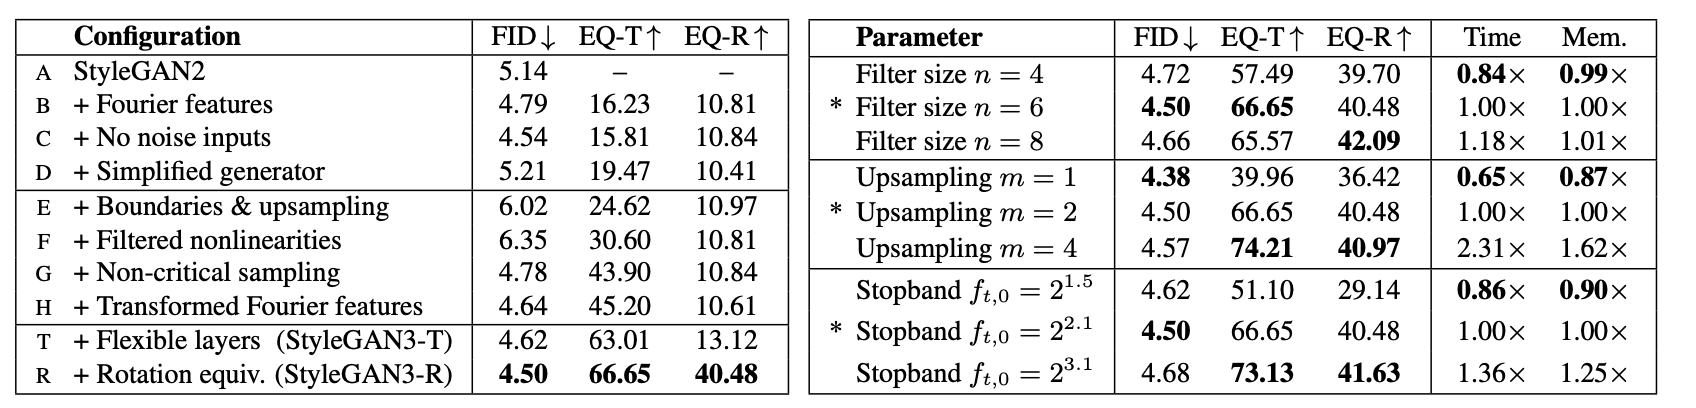
\includegraphics[width=0.9\textwidth]{img/m2t21.png} 
\caption{FID 在 50k 图像和所有训练图像计算}
\label{Test}
\end{figure}

如图下所示当中(a)绿色的过渡带更宽,减少不必要的阻带纹波,从而导致更强的衰减。而(b)StyleGAN3,对应于上图中的 configs t 和 r。主要的数据通路包括傅里叶特征和归一化,调制卷积,以及非线性过滤器。

\begin{figure}[htb]
\centering 
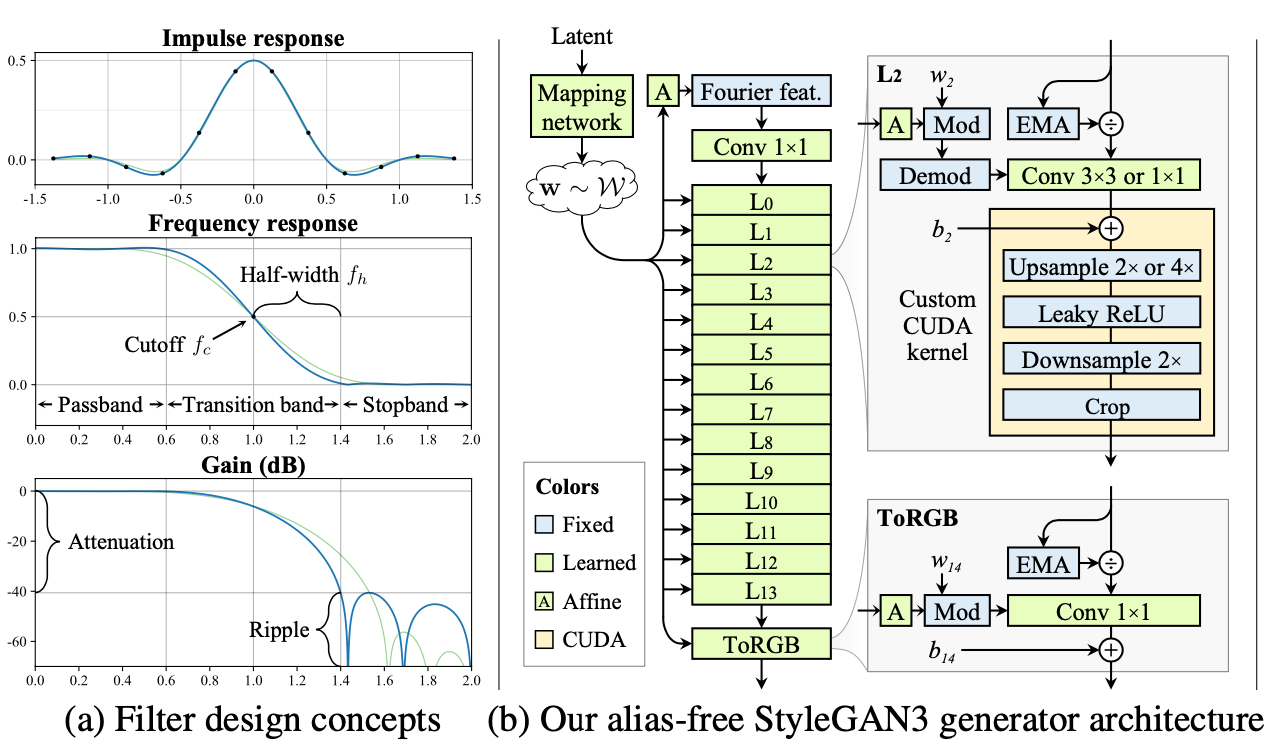
\includegraphics[width=0.9\textwidth]{img/m2t22.png} 
\caption{StyleGAN3 说明}
\label{Test}
\end{figure}

而 StyleGAN3 与过往 styleGAN2 相比,具有下列四项新特性:

\begin{enumerate}
 \item [-] Alias-free 生成器架构和训练配置(stylegan3-t 和 stylegan3-r);
 \item [-] 提供交互式可视化(visualizer.py)、频谱分析(avg\_spectra.py)和视频生成(gen\_video.py)的工具;
 \item [-] 同变性度量(eqt50k\_int、 eqt50k\_frac 和 eqr50k);
 \item [-] 其他改进:减少内存使用、训练速度略升以及 bug 修复。
\end{enumerate}

3. 结论和未来展望
StyleGAN2 生成的动物毛发会粘在屏幕上,和动物的形态变化不一致。这就是StyleGAN变体一直无法解决的难题之一。它从根本上解决了StyleGAN2 图像坐标与特征粘连的问题,实现了真正的图像平移、旋转等不变性,大幅提高了图像合成质量,而在 GAN 的相关文献中,混叠这一概念很少被提及,研究者在这项研究中,提供了两个混叠来源 :1)由非理想上采样滤波器(如卷积、双线性卷积或跨步卷积)产生的像素网格后模糊图像。2)非线性的逐点应用,如 ReLU 或 swish 。
他们发现,混叠网络具有放大并在多个尺度上组合图像像素的能力,这对于弱化固定在屏幕坐标中的纹理图案至关重要。并且实验证明,该网络还适用于深度学习中所有常用过滤器,甚至图像处理中使用的高质量过滤器。
本研究知道,成功消除所有位置参考来源意味着无论像素坐标如何,细节都可以被很好地生成,它相当于在所有层中对亚像素平移(和旋转)实施连续的等方差。而事实证明,当前的上采样滤波器在抑制混叠方面根本不够积极,而且需要具有超过100dB衰减的高质量滤波器。这项研究提出了一种解决点态非线性引起的混叠的原理,考虑了它们在连续域的影响,并对结果进行适当的低通滤波。
此外,实验证明:一个基于1×1卷积的模型能够产生强旋转的等变生成器。一旦适当地抑制了混叠以迫使模型实现更自然的层次细化,它的操作模式就会发现显著变化:坐标系统等内部表示,允许细节准确地附加到底层表面。这将显著改进用于生成视频和动画的模型。 另外值得注意的是,英伟达的 StyleGAN3 项目消耗了令人难以想象的资源和电力。研究者在论文中表示,整个项目在 NVIDIA V100 内部集群上消耗了 92 个 GPU year(即单个 GPU 一年的计算)和 225 兆瓦时(Mwh)的电力。而在社会影响方面,GANs 的潜在负面社会影响包括许多形式的虚假信息,例如社交媒体上的虚假肖像,甚至领导人的宣传视频,而本论文的结果将会消除那些视频中的人造痕迹,潜在地让视频更有说服力,或者说更有欺骗性。

\section{预训练图像生成模型的应用}

\subsection{GAN Inversion: A Survey}

研究者先是交代了 GAN 的重要性与概述,同时并说明 GAN inversion 的在给定的影像反转预训练的 GAN 模型潜在空间,好方便生成器可以反转得作用,另外研究者也全面性的调查近几年在  GAN inversion  相关的研究、应用与贡献,该项研究工作是首次对 GAN 反演 的第一次调查,并且该研究团队在此领域的所有方面做出全面系统的回顾和分析,同时在完成分析后对该 GAN 反演方法中的属性与性能做出比较总结,最后并确定该领域所面对的挑战与问题,并确定对于未来研究的趋势。

随后研究者针对 GAN 反转的问题定义和概述进行详细的说明,其众所周知 GAN 能够生成高分辨率和逼真的“假”图像,但鲜为人知的一个方面是如何将这些 GAN 应用在“真实”图像上。而第一种可能的解决方案,该篇研究的重点,亦即 GAN 反演,是获取“真实”图像的潜在代码,并通过操纵潜在空间中的潜在代码来执行一些后续的图像处理任务。而 GAN 反演将会试图找到一个潜在的代码,并为给定图像实现两个目标,其一为忠实地和逼真地重建输入图像,首先运用数学做好定义,并条件映射找到视觉相似的对应图像,其二则是做促进下游的任务,而所谓的下游任务的目标又取决于使用哪一个潜在空间。同时研究也说明,往常像是面部图像为例且基于学习的 GAN 反演方法不能忠实地重建图像内容,即便基于优化的技术已经实现了卓越的图像重建,但它们不可避免的缺点是计算成本显著地增加。所以基于学习的 GAN 反演方法的最新改进主要集中在如何忠实地重建图像,例如在训练资料时或提出迭代反馈机制来整合额外的面部身份损失。另外在基于优化的方法的最新改进更加强调如何更快地找到所需的潜在代码,并提出了几种关于初始化和优化器的策略。诚然现有的反演方法无法同时实现重建质量和推理时间,从而导致“质量-时间权衡”(quality-time tradeoff),尽管另外提出了一些混合方法来平衡这种权衡,但快速找到准确的潜在代码仍然是一个挑战。

研究者整理出近期广泛应用如下 :

\begin{enumerate}
 \item [-] 图像处理 (Image Manipulation)
 \item [-] 图像生成 (Image Generation)
 \item [-] 图像修复 (Image Restoration )
 \item [-] 图像插值 (Image Interpolation)
 \item [-] 风格转移 (Style Transfer)
 \item [-] 压缩感知 (Compressive Sensing)
 \item [-] 语义扩散 (Semantic Diffusion)
 \item [-] 品类转移 (Category Transfer) 
 \item [-] 对抗性防御 (Adversarial Defense)
 \item [-] 3D 重建 (3D Reconstruction)
 \item [-] 图像理解 (Image Understanding)
 \item [-] 多模态学习 (Multimodal Learning)
 \item [-] 医学影像 (Medical Imaging)
\end{enumerate}

而在研究中,研究者们提出在该领域的挑战和未来方向如下 :

1. 理论理解 (Theoretical Understanding)

尽管在应用上取得了成功,但对 GAN 反演仍缺乏理论认识且 GAN 反演可以被视为与 PCA 通常执行的降维的非线性等效。数据中的非线性结构可以紧凑地表示,并且诱导几何需要使用非线性统计工具、黎曼流形和局部线性方法。相关领域的成熟理论可以从不同角度促进对神经网络权重(参数)或潜在空间方面的 GAN 反演的更好的理论理解。例如,研究可以将 GAN 反演公式化为将信号分解为分量(矩阵分解问题),并使用非线性因子分析 (FA)、独立分量分析 (ICA)和潜在狄利克雷分配 (LDA) , 分解网络权重并找到潜在空间的可解释方向。

2. 反转类型 (Inversion Type)

除了 GAN 反转之外,还开发了一些方法来反转基于编码器-解码器架构的生成模型。 IIN 方法学习变分自编码器 (VAE) 的可逆解开解释。 Zhu et al. 开发了潜在可逆的自动编码器方法来学习人脸图像的解开表示,可以根据属性从中编辑内容。而 The LaDDer approach 使用基于生成先验(包括加性 VAE 和超先验混合)的元嵌入将训练有素的 VAE 的潜在空间投影到低维潜在空间,其中使用多个 VAE 模型 形成层次化的表示。探索如何结合 GAN 反演和编码器解码器反演是有益的,这样研究就可以利用到两全其美。

3. 域泛化 (Domain Generalization) 

GAN 反演已被证明在跨域应用中是有效的,例如风格迁移和图像恢复,这表明预训练模型已经学习了域不可知的特征,来自不同域的图像可以倒置到相同的潜在空间中,从中可以得出有效的度量。目前已经开发出多任务方法来协同利用视觉线索,例如 GAN 框架内的图像恢复和图像分割或语义分割和深度估计。

4. 场景表示 (Scene Representation)

GAN 反演方法可以操纵几何(例如,缩放、移位和旋转)、纹理(例如,背景模     糊和锐度)和颜色(例如,照明和饱和度)。这种能力表明在大规模数据集上预训练的 GAN 模型已经从现实世界的场景中学到了一些物理信息。隐式神经表征学习是 3D 社区的最新趋势,它学习 3D 形状或场景的隐式函数,并能够控制场景属性,例如照明、相机参数、姿势、几何形状、外观 , 和语义结构。它已用于体积性能捕获、新视图合成、面部形状生成、对象建模和人体重建。最近的 StyleRig 方法是基于 3D 可变形模型 (3DMM)的语义参数和 StyleGAN 的输入进行训练的。它开辟了一个有趣的研究方向,以反转用于 3D 重建的预训练 GAN 的这种隐式表示,例如,使用 StyleGAN 进行人脸建模或延时视频生成。

5. 精确控制 (Precise Control)

GAN 反演可用于找到图像处理的方向,同时保留身份和其他属性,诚然这还需要一些调整来实现精确细粒度控制的所需粒度,例如注视重定向、重新照明和连续视图控制。

6. 多峰倒置 (Multimodal Inversion)

现有的 GAN 反演方法主要涉及图像。然而,生成模型的最新进展超出了图像领域,例如用于音频合成的 GPT-3 语言模型和 WaveNet。这些复杂的深度神经网络经过各种大规模数据集的训练,已被证明能够表示广泛的不同内容、风格、情感和主题。在这些不同的模态上应用 GAN 反转技术可以为语言风格转移等任务提供新的视角。

7. 评估指标 (Evaluation Metrics)

感知质量指标可以更好地评估逼真和多样化的图像或与原始图像一致的身份,仍有待探索。此外,评估主要集中在照片写实度上,或者使用针对真实图像训练的模型判断生成图像的分布是否与真实图像在分类或分割准确性方面一致。然而,仍然缺乏有效的评估工具来评估预测结果与预期结果之间的差异或更直接地衡量倒置的潜在代码。

\subsection{Encoding in Style: a StyleGAN Encoder for Image-to-Image Translation}

1. 背景和动机
GAN 的提出对于图像生成,尤其是对与人脸相关的图像生成任务有显著的提升。英伟达在此基础上提出了 StyleGAN ,引入了风格向量来更好地编码输入图像。原有的   隐空间 z 中的特征之间相互关联、耦合,而经过多层感知机映射到新的隐空间w之后,特征之间更加独立,更方便对特征进行可视化控制。
本文基于的是 StyleGAN 升级后的 StyleGAN2 ,并提出了一个可以直接将真实人脸图像直接映射到 W+ 隐空间的 encoder 。 StyleGAN2 主要对 AdaIN 作了修改,解决了 StyleGAN 生成的图像中存在伪影的问题,并对生成图像的质量作了进一步的提升。

2. 本文主要贡献

(1) 本文提出了一个能将真实人脸图像直接映射到W+隐空间的encoder。

(2) 本文提出了一个通用的解决 image2image 问题的 pSp 端到端框架。

\begin{figure}[htb]
\centering 
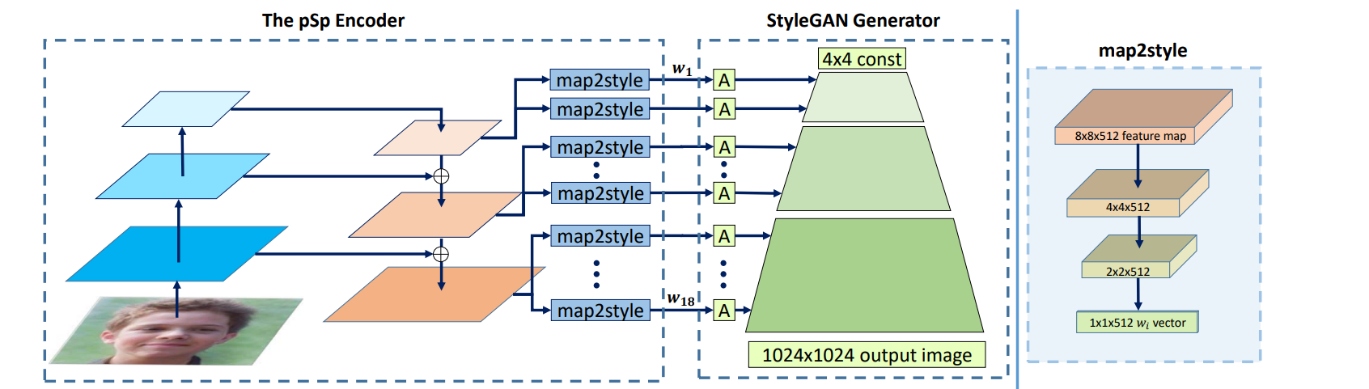
\includegraphics[width=0.9\textwidth]{img/m2t23.png} 
\caption{pSp 端到端框架}
\label{Test}
\end{figure}

pSp 框架基于新型编码器网络,该网络生成一系列 style 向量,然后输入到预训练的 StyleGAN 中,形成扩展的 W+ 。首先,该编码器可以直接将真实图像嵌入到 W+ 中,无需额外优化。其次,编码器可以直接解决图像的转换任务,即图像转换任务定义为:从输入域到潜在域的编码问题。与先前使用 “先反转,后编辑” 的方法不同,pSp 不要求输入图像在 StyleGAN 域中进行特征表示,也可以处理各种任务。该编码器极大地简化了训练过程,在没有图像对的标签下提供更好的支持,并且通过 style 的重采样可以支持多模态合成。最后,pSp 的应用不仅限于人类面部领域,即使与专为特定任务而设计的解决方案相比,也表现极佳。

3. 实验结果

(1) StyleGan inversion 任务

首先评估了 pSp 框架在 StyleGan inversion 任务上的效果,尤其在 latent domain 中发现真实图片的 latent code。并且将论文的方法与 Karras 的优化技术进行比较,當中包含了 ALAE 编码器和 IDInvert 编码器,其中 ALAE 是一种基于 StyleGan 的自动编码器,编码器和生成器一起训练以生成 latent codes。而对于 IDInvert,图像被嵌入到一个预训练的latent domain中:首先,图像被编码到 W+ 中,然后直接对生成的图像进行优化以调整latent。为了进行公平的比较,论文与IDInvert进行比较,并且在编码后不再做进一步的优化。从结论来说,在对输入图像的重建任务上,ALAE效果较差,IDInvert 能较好的保留图像
属性,但不能准确地保留人脸的一致性。而论文的 pSp 更加真实,能保留更细节的属性:比如灯光、发型、眼镜。

(2) 人脸正面化实验

由于需要非局部变换以及缺少成对数据的问题,人脸正面化难度还是很大的,RotateAndRender 通过 3D 几何对齐来解决这个问题。论文是直接生成,甚至用没有标记的数据训练。而方法主要有两个额外的操作,一个是在训练过程中针对target图像进行随机flip,这样迫使网络学习一个中间位置,也就是正面的脸,保证正面化前后人脸的一致性。二是由于此研究并不是太关注图像的背景信息,因此从loss部分进行了一些权重的调整,主要是 L2 和 LPIPS。

而从结论来看,pix2pixHD 不能收敛到一个比较优秀的结果,因为 pix2pixHD 很大程度上依赖条件因素中的成对信息。该论文的 pSp 方法能较好保持人脸原有属性,同时将其成功转化为正脸,与  RotateAndRender 方法的效果相当,但 pSp 方法更简单,不需要一些专门的模块,比如 R\&R 的 3DMM安装和喷涂步骤。

(3) 其他任务上的拓展

PULSE 给出了一个从 LR 到 HR 的生成式的超分方案:将 HR 图像的 manifold 下采样到 LR 的大小,然后通过计算损失来优化输入的无监督方式。pSp 也再这方面做出了一些尝试,可以获得和 PULSE 相比不错的结果。pSp 使用了全监督的方式来进行训练,针对输入随机进行采样 x1,x2,x4,x8 和 x16 然后插值放大到原始大小。pix2pixHD 给出了不错的结果,但是 less photo-realistic;PULSE能生成高精度图像,但是不那么像原来的那个人了。然后,针对 medium 的层设置 $\alpha = 0.5$ 做 style mixing,控制面部特征,而 pSp 也可以生成多个结果。

4. 结论以及展望

这篇论文提出了一种新的编码器体系结构,它可以用来直接将真实图像映射到W+潜在空间,而不需要优化。在这种结构中,样式以分层方式提取,并被提供给固定 StyleGAN 生成器的相应输入。结合编码器和 StyleGAN 解码器,作者提出了一个通用的框架来解决各种图像到图像的转换任务,所有这些任务都使用相同的架构。值得注意的是,与以前 StyleGAN 编码器的“先反转,后编辑”方法不同,作者展示了 pSp 可用于将这些翻译任务直接编码到 StyleGAN 中,从而支持不在 StyleGAN 域中的输入图像。此外,与以往的工作不同的是,以前的工作通常依赖于专用的架构来解决单一的翻译任务,而作者通过实验pSp能够解决各种各样的问题,只需要对训练损失和方法进行最小程度的改变。下一步研究者可以研究利用 StyleGAN 进行真实图像到图像的翻译任务。

\subsection{A Style-Based Generator Architecture for Generative Adversarial Networks}

1. 论文简介

本文从风格转换文献中提出了一种生成对抗网络的可替代生成器框架。新的框架导致了高级属性(如人脸训练时的姿势和身份)的自动学习和无监督分离,以及生成图像中的随机变化(如雀斑、头发),并实现了对合成的直观、特定规模的控制。新的生成器在传统分布质量指标方面改进了目前最先进的技术的效果,有明显更好的插值特性,也更好地解耦变量的潜在因素。为了量化插值质量和解耦效果,此研究提出了两种新的、自动化的方法,适用于任何生成器架构。最后,本文构建了一个新的、高度多样化和高质量的人脸数据集。

2.研究背景

生成方法产生的图像的分辨率和质量——特别是生成对抗网络(GAN)——最近得到了快速的改善。然而,这些生成器仍然像黑盒子一样运行,尽管最近的努力,对图像合成过程的各个方面的理解,例如,随机特征的起源,仍然缺乏。潜在空间的性质也没有得到很好的理解,常用的潜在空间插值没有提供定量的方法来比较不同的生成器。

受风格转换文献的启发,该研究重新设计了生成器的架构,以提出新的方法来控制图像合成过程。研究的生成器从一个学习过的常量输入开始,根据潜码在每个卷积层调整图像的“风格”,从而直接控制不同尺度下图像特征的强度。与直接注入网络的噪声相结合,这种架构上的变化导致生成图像中的高级属性(例如姿态、身份)与随机变化(例如雀斑、头发)自动、无监督地分离,并实现了直观的特定尺度的混合和插值操作。研究不以任何方式修改判别器或损失函数,因此该研究的工作与正在进行的关于 GAN 损失函数、正则化和超参数的讨论是正交的。

研究者将的生成器将输入的潜在编码嵌入到一个中间的潜在空间中,这对变量因子在网络中的表现方式有着深远的影响。输入潜在空间必须遵循训练数据的概率密度,此研究认为这导致了某种程度的不可避免的纠缠。研究的中间潜在空间中就不受这个限制,因此可以解耦合。由于之前估计潜在空间解耦程度的方法不能直接应用于本研究的案例,本研究提出了两个新的自动化度量方法——感知路径长度和线性可分性——来量化生成器的这些方面。使用这些指标,本研究表明,与传统的生成器架构相比,本研究的生成器实现了一个在不同变量因素中能得到更线性,更少耦合表现的效果。

最后,研究者们提供了一个新的人脸数据集(Flickr-Faces-HQ, FFHQ),它比现有的高分辨率数据集提供了更高的质量,涵盖了更广泛的变化。同时研究者将这个数据集,连同此研究的源代码和预先训练好的网络一起公开。

\begin{figure}[htb]
\centering 
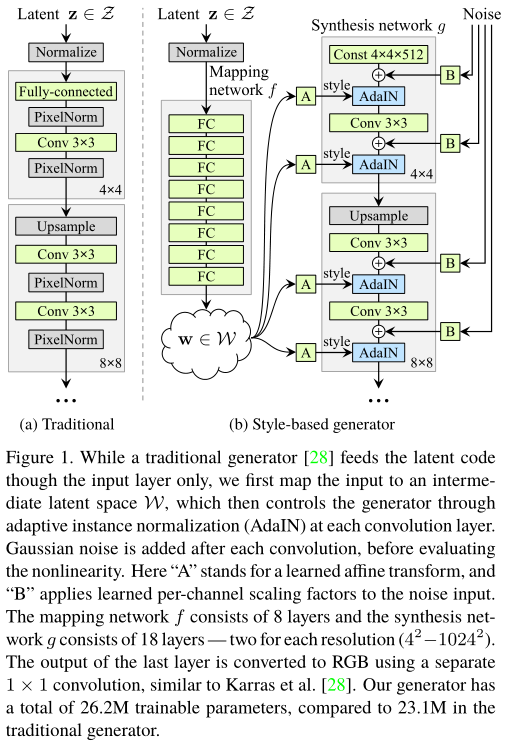
\includegraphics[width=0.9\textwidth]{img/m2t24.png} 
\caption{Style-Based Generator}
\label{Test}
\end{figure}

3. Style-based generator

通常潜在编码通过输入层提供给生成器,即前向网络(图1a)的第一层。研究者通过省略该输入层和从一个可学习常量(图1b,右)开始来分离该设计。给定一个在输入潜在空间Z的潜在编码z、一个非线性的映射网络 $f:\mathcal{Z}\rightarrow\mathcal{W}$来生成$w\in\mathcal{W}$(图 1b,左)。简单来说,研究设置两个空间的维度为 512(即 Z 和 W 都是 512x1),映射函数 f 使用 8 层 MLP 来实现,决策函数将在 Section 4.1分析。可学习的仿射转换(A)将 w 转换成 styles $y=\left(y_s,y_b\right)$ ,用来控制生成网络 g 每一个卷积层后面的 adaptive instance    normalization(AdaIN)操作。该 AdaIN 操作被定义为:

\begin{equation}
AdaIN\left(x_i,y\right)=y_{s,i}\frac{x_i-\mu\left(x_i\right)}{\sigma\left(x_i\right)}+y_{b,i}
\end{equation}

每个特征映射 $x_i$ 将会被分别归一化,然后使用来自style y的对应尺寸成分 $y_{s,i}$ 和 $y_{b,i}$ 来按比例变化和实现偏差。因此,y 的维数是该层上特征图数量的两倍。
将此研究的方法与风格转移相比较,本研究从向量 w 中计算空间不变风格y,而不是从一个例子图像中计算。而此研究选择对 y 重复使用“style”这个词是因为类似的网络架构已经被用于前向风格传输、无监督图像到图像的转换和域混合中。与更一般的特征变换相比, 因为 AdaIN 的效率和紧凑的表示,其特别适合此研究的目的。简单说明下这个网络,在潜在编码 Z 中间添加一个 mapping 网络,用来将输入的向量编码为中间向量 W,然后该中间向量将会分别传送 18 个控制向量 A 到生成网络 g 中的 18 层上,用来控制不同的 style。
而要加 Mapping Network 的原因在於,后续得到的18个控制向量之间会存在特征纠缠的现象——比如说研究想调节 8*8 分辨率上的控制向量(假设它能控制人脸生成的角度),但是此研究会发现32 * 32 分辨率上的控制内容(譬如肤色)也被改变了,这个就叫做特征纠缠。所以Mapping Network的作用就是为输入向量的特征解缠提供一条学习的通路。最后就能够使用上面(图1b)输出的1024*1024的图像和真正图像作为 Discriminator 的输入,最小化损失来训练模型参数,而最后我們提供了一个直接的方法,通过引入显式噪声 noise 输入以产生随机细节。这些是由不相关的高斯噪声组成的单通道图像,本研究为合成网络的每一层提供一个专用的噪声图像。利用学习到的每个特征的缩放因子将噪声图像广播到所有的特征映射上,然后加入到相应卷积的输出中。

4. 生成效果

在研究该研究的的生成器的特性之前,此研究通过实验证明,重新设计不会影响图像质量,但实际上,它大大改善了图像质量。表中给出了各种生成器架构在数据 CELEBA-HQ 和在研究者的新 FFHQ 数据集上的 Frechet inception distances(FID)效果。此研究的 baseline 配置(A)是 Karras et al. 的 Progressive GAN 设置, 除非另有说明,否则此研究继承了网络和所有超参数。首先研究者通过使用双线性上/下采样操作、更长时间的训练和调优超参数来切换到改进的baseline(B)。训练设置的详细描述和超参数包含在附录C中。然后本研究通过添加映射网络和AdaIN操作进一步改善这一新的baseline(C),并得到一个令人惊讶的发现,即网络不再受益于将潜在编码输入到卷积第一层的这个操作。因此本研究通过消除传统的输入层和开始从一个可学习的 4×4×512 常量张量开始图像合成来简化架构(D,因为StyleGAN生成图像的特征是由W和AdaIN控制的)。 本研究发现一个很了不起的效果,即合成网络能够产生有意义的结果,尽管它接收输入只有用来控制 AdaIN 操作的 style。

\begin{figure}[htb]
\centering 
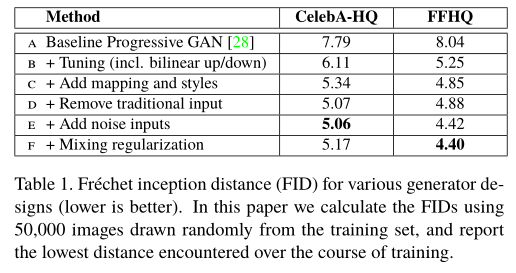
\includegraphics[width=0.9\textwidth]{img/m2t25.png} 
\caption{生成效果}
\label{Test}
\end{figure}

最后,此研究引入了进一步改善结果的噪声输入(E,noise inputs),以及新的混合正则化(F,mixing regularization),它去除了邻近的style,并对生成的图像进行更细粒度的控制。此研究使用两种不同的损失函数来评估本研究的方法:对于CELEBA-HQ,本研究依赖于 WGAN-GP,而 FFHQ 使用 WGAN-GP 来处理配置 A,对于配置B-F,使用R1正则化的非饱和损失。本研究发现这些选择可以得到最好的结果。该研究的贡献不改变损失函数。同時此研究观察到,对比传统的生成器(B),基于风格的生成器(E)很明显地改进了FIDs,几乎提高了20\%,这证实了在并行工作中进行的大规模ImageNet测量。经FIDs确认,平均质量高,甚至连眼镜、帽子等配件都成功合成。

5. 生成器的特性

此研究的生成器架构,使它能够通过特定比例的 style 修改来控制图像合成。本研究可以把映射网络和仿射变换看作是一种从学习分布中为每种风格抽取样本的方法,而合成网络则是一种基于 styles 集合来生成新图像的方法。每种 style 的效果在网络中都是局部的,即修改 style 的特定子集只能影响图像的某些方面。

为了了解这种定位的原因,让本研究考虑一下 AdaIN 操作如何首先将每个通道归一化为零均值和单位方差,然后根据 style 应用尺度和偏差。根据 style,新的每个通道统计信息修改了后续卷积操作中特征的相对重要性,但由于归一化,它们不依赖于原始统计信息。因此,每种 style 在被下一个 AdaIN 操作覆盖之前只能控制一个卷积

6. 风格混合

为了进一步鼓励 style 的定位,本研究采用 mixing regularization,即在训练过程中使用两个随机的潜码生成给定百分比的图像。当生成这样的图像时,本研究只需要在合成网络中随机选择的一个点从一个潜在代码切换到另一个——该研究称之为 style mixing 的操作。具体来说,本研究通过映射网络运行 z1、z2 这两个潜码,然后就有对应的 w1、w2 控制 style,将w1应用在交点之前,w2应用在交点之后。这种正则化技术防止网络假设相邻样式是相关的。

7. 结论

基于该研究的结果和 Chen 等人的并行工作,传统的 GAN 生成器体系结构在各个方面都不如基于风格的设计。就已建立的质量度量而言,这是正确的。研究者进一步相信,研究者对高阶属性和随机效应的分离以及中间潜在空间的线性的研究将证明在提高GAN合成的理解和可控性方面卓有成效。而研究的平均路径长度度量可以很容易地在训练期间用作正则化器,也许线性可分度度量的某些变体也可以用作正则化器。总的来说,研究者期望在训练过程中直接塑造中间潜在空间的方法将为未来的工作提供有趣的途径。

\subsection{ReStyle: A Residual-Based StyleGAN Encoder via Iterative Refinement}

1. Topic:图像反演,获取潜在编码用于对图像进行直接编辑。

2. Problem:现在的单次编码架构无法准确的获得图像反推的潜在编码。即在重建精度方面,基于学习的反演方法与基于优化的反演方法仍存在较大差距。因此,虽然在基于学习的反演方面取得了显著的进展,但设计合适的编码器和训练方案仍然是一个挑战,许多工作仍在使用逐图像优化方法。

3. Idea:使用以残差为基础的迭代反馈调优架构。具体为将上一次迭代的输出与原始的输入图像共同输入到下一次迭代中,进行多次前向传播,让编码器注意到更多能够提升精度的特征。在增加有限的推理时间情况下,实现较高精度的输出。个人理解该方法是逐图像优化方法与编码器学习方法的折中。也是单步反演的松弛求解。

\begin{equation}
\hat{y}=G(E(x))
\end{equation}
其中 $x$ 为输入图像,$\hat{y}$ 为反演的图像,G, E 分别为生成器和编码器。

4. Methods:

\begin{enumerate}
 \item [-] 聚合真实图像和Stylegan的重建图像,生成六通道数据,然后输入到编码器中学习残差偏移编码
 \item [-] 更新图像x的潜在编码,并输入到生成器中生成新重建图像
 \item [-] 其中初始的潜在编码和对应的潜在图像分别是训练好的生成器的平均风格向量和其对应生成图片
\end{enumerate}

5. 模型 :

\begin{figure}[htb]
\centering 
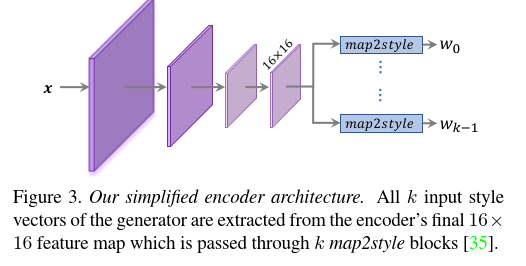
\includegraphics[width=0.9\textwidth]{img/m2t26.png} 
\caption{ReStyle}
\label{Test}
\end{figure}

6. 编码器模型:因为迭代调优的特性,SOTA工作中的特征金字塔和残差模块在该网络中并不需要。文中采用简单的特征下采样网络并结合StyleGAN的需要的风格输入作为输出,如上图。

7. 实验:该作者对于不同的图片域进行了模型评估,分别是人脸域,汽车域和其他GAN常用的图片域数据集。

8. 图像反演的效果:虽然与基于学习的方法相比,逐图像优化技术实现了更好的图像重建,但它们带来了显著更高的计算成本。因此,在分析反演方法时,必须根据推断时间来衡量重建质量,从而导致所谓的质量-时间权衡。

\begin{figure}[htb]
\centering 
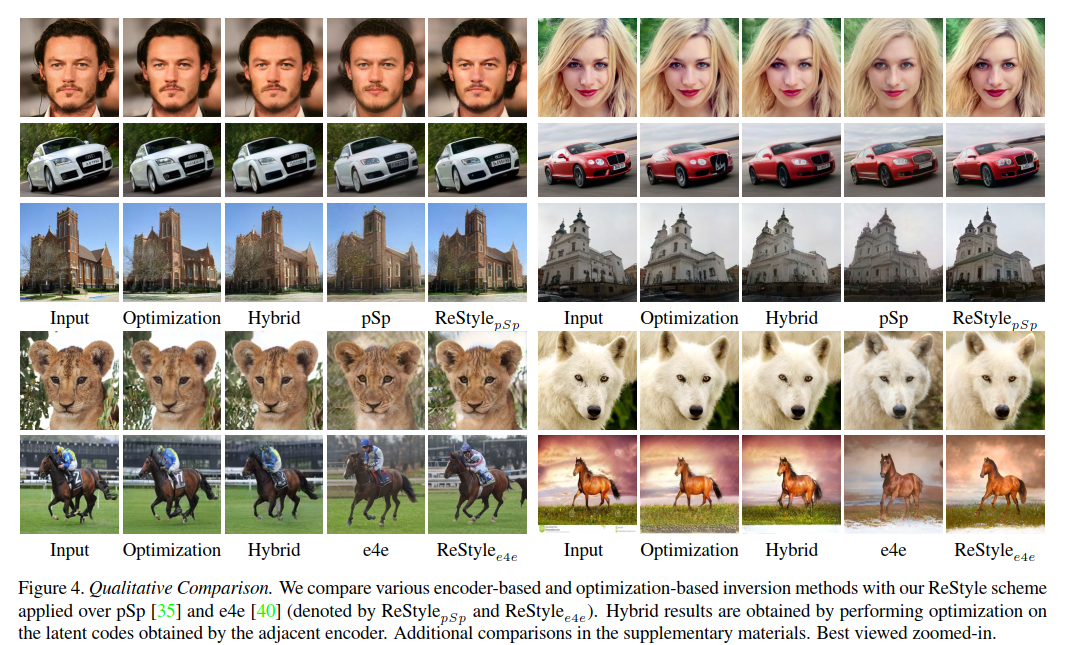
\includegraphics[width=0.9\textwidth]{img/m2t27.png} 
\caption{ReStyle}
\label{Test}
\end{figure}

9. 定性分析:相比于e4e和psp,所提出模型能够逼近逐图像优化和真实值。研究从分析面部区域开始。与传统的pSp和e4e编码器相比,该研究的ReStyle变体可以匹敌或超过它们的对手。更值得注意的是,虽然与ReStyle相比,优化技术实现了更好的身份相似性,但它们需要20多时间来匹配ReStyle获得的相似性。在汽车领域也可以观察到类似的权衡,在评估重构L2损失时,ReStyle相对于典型编码器的优势更加明显。在非结构化教堂领域,应用在pSp上的ReStyle在重构质量上与优化和混合技术几乎一致,且推断时间显著降低。虽然优化通常可以实现卓越的重构,但ReStyle在重构质量和推断时间之间提供了极佳的平衡。

10. 图像 restyle 过程与效果:在早期的步骤编码器专注于精炼的背景和姿势,而在随后的步骤编码器移动其焦点调整更精细的细节沿着眼睛和头发。编码器的工作方式从粗到精,从集中于低频细节开始,然后逐渐通过调整高频细节来补充。

\begin{figure}[htb]
\centering 
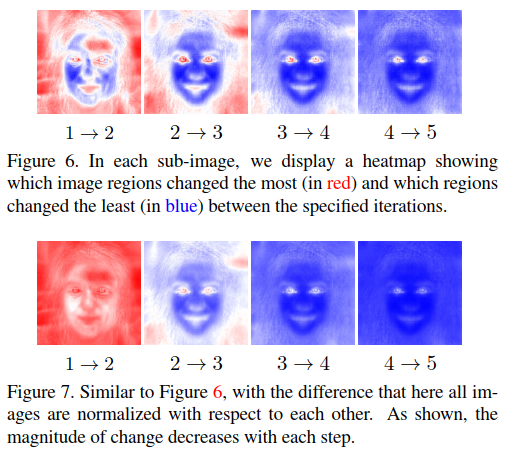
\includegraphics[width=0.9\textwidth]{img/m2t28.png} 
\caption{图像 restyle 过程与效果}
\label{Test}
\end{figure}

11. 结论:该文章提出了一个用于图像反演,编辑和美化的通用框架。

\subsection{Designing an Encoder for StyleGAN Image Manipulation}

1. 背景和动机

本文的目的是为了设计编码器能够更好的对图像进行编辑。首先,由于图像失真,感知质量和图像的可编辑性存在紧密的连系。在一定程度上,图像失真与感知质量存负相关,图像失真和图像的可编辑性成负相关。此外,本文还发现如果图像的逆隐空间向量越接近原本的隐空间分布W,那么图像的感知质量和可编辑性便越好。

2. 本文主要贡献

\begin{enumerate}
 \item [-] 分析了 StyleGAN 复杂的隐空间并且提出了一个创新的结构
 \item [-] 分析并讨论了图像失真,图像感知和可编辑性之间的权衡
 \item [-] 对这些权衡进行了分析,并且设计了两种方法来实现控制器来控制他们
 \item [-] 提出了 e4e ,一个创新的编码器专门设计来允许对反转真实图像的接下来的编辑。
\end{enumerate}

3. 实验结果

实验采用了 2 种配置,配置A没有采用d-reg和 $D_W$ 损失,而配置 D 采用d-reg和 $D_W$ 两种损失。首先分析了两种配置下的生成 latent vector 哪一种更接近 W。采用计算各个 latent style code 的方差来判断是否相近。最终配置 D 比配置 A 明显更小。说明配置D生成的明显比配置A更要接近W。在失真的评估上,配置 A 要优于配置 D。而在感知质量和可编辑性上,FID 和 SWD 两种评估指标之间互相矛盾,因为这两个评估指标均不能准确的给出评估。最后本文采用人类评估的调查来评估感知质量和可编辑性。从调查中不难发现,配置 D 的效果在这两方面要远优于配置 A 。最终可以得出,配置 D 的方法要更接近于 W,虽然增大了一定程度的失真,但是该方法会让感知质量和可编辑性有所降低。

